\RequirePackage{luatex85}
\documentclass[12pt, bibliography=totoc, listof=totoc, svgnames]{scrreprt} 	% Beginn Dokument
\usepackage{cite}				% Fürs Zitieren
\usepackage[utf8]{inputenc} 	% Verwendete ASCII Codierung für ä ö ü
\usepackage[dvips]{graphicx}	% Für Graphen
\usepackage[english]{babel} 		% Englisch als Sprache
\selectlanguage{english}
\usepackage{amssymb}
\usepackage{listings}
\usepackage{color}
\usepackage{gensymb}
\definecolor{mygreen}{rgb}{0.8,0.8,0.8}
\lstset{backgroundcolor=\color{mygreen}}

\usepackage[footnote]{acronym}
%\renewcommand*\bflabel[1]{{\textbf{\textsf{#1}}\dotfill}}
%\renewcommand*{\acsfont}[1]{{\color{black}\textit{#1}}}

\usepackage{todonotes}

%%% Papierformat %%%
\usepackage{geometry}			
\geometry{a4paper}
\geometry{paper=a4paper,left=30 mm,right=30 mm,top=30 mm}

%%% Packages für den Graphen %%%
\usepackage{pgf}
\usepackage{tikz}
\usetikzlibrary{arrows,automata}
\setlength{\parindent}{0mm}
\usepackage{booktabs}
%%% Kopf & Fußzeilen %%%
\usepackage{fancyhdr} % This should be set AFTER setting up the page geometry
\pagestyle{fancy} % options: empty , plain , fancy
\fancypagestyle{plain}{}% damit auch "plain" Seiten fancy werden
\renewcommand{\headrulewidth}{1pt} % customise the layout…
\lhead{\textsc{Robot Control Report}\\
%\emph{\leftmark}
}\chead{}\rhead{}
\lfoot{}\cfoot{}\rfoot{\thepage}
\setlength{\headheight}{40pt}
\renewcommand*{\chapterheadstartvskip}{\vspace*{.1\baselineskip}}% Abstand einstellen

%%% HRule erzeugt eine Linie nach einem Absatz %%%
\newcommand{\HRule}{\rule{\linewidth}{0.5mm}}



\usepackage{tabularx}
\usepackage{amsmath}

\usepackage{xcolor}
\usepackage{verbatim}

\bibliographystyle{unsrt}

\begin{document}
%\maketitle

\begin{titlepage}

\begin{center}


% Upper part of the page
	%\includegraphics[width=0.60\textwidth]{pics/FH}\\[1cm]    
	\begin{tikzpicture}[font=\sffamily]
	\node [circle] (dot1) {};
	\node [circle] (dot2) at ($(dot1.west) + (-0.4, 0)$) {};
	\node [circle] (dot3) at ($(dot1.east) + (+0.4, 0)$) {};
	\node [circle] (dot4) at ($(dot2.north) + (0, 0.4)$) {};
	\node [circle] (dot5) at ($(dot3.north) + (0, 0.4)$) {};
	\node [circle] (dot6) at ($(dot2.south) + (0, -0.4)$) {};
	\node [circle] (dot7) at ($(dot3.south) + (0, -0.4)$) {};
	
	\node [circle] (fdot1) at ($(dot1) + (-2, 0)$) {};
	\node [circle] (fdot2) at ($(fdot1.west) + (-0.4, 0)$) {};
	\node [circle] (fdot3) at ($(fdot1.north) + (0, 0.4)$) {};
	\node [circle] (fdot4) at ($(fdot2.south) + (0, -0.4)$) {};
	\node [circle] (fdot5) at ($(fdot2.north) + (0, 0.4)$) {};
	\node [circle] (fdot6) at ($(fdot3.east) + (0.4, 0)$) {};
	
	\draw [ultra thick] ($(fdot5.north west)+(-0.5, 0.6)$) -- ($(fdot4.south west)+(-0.5, -0.6)$);
	
	\node [red!80!black, text width=2.6cm, align=flush center] (text1) at ($(fdot1) + (-2.9, 0.6)$) {\textbf{C\hfill A\hfill R\hfill I\hfill N\hfill T\hfill H\hfill I\hfill A}};
	\node [text width=2.6cm, align=center] (text2) at ($(text1.south) + (0, -0.13)$) {\textbf{U\hfill N\hfill I\hfill V\hfill E\hfill R\hfill S\hfill I\hfill T\hfill Y}};
	\node [text width=2.6cm, align=center] (text3) at ($(text2.south) + (0, -0.13)$) {\textbf{O\hfill F \hfill A\hfill P\hfill P\hfill L\hfill I\hfill E\hfill D}};
	\node [text width=2.6cm, align=center] (text4) at ($(text3.south) + (0, -0.13)$) {\textbf{S\hfill C\hfill I\hfill E\hfill N\hfill C\hfill E\hfill S}};
	
	\node [text width=5cm, align=center] (text5) at ($(dot4.west) + (2.5, 0.6)$) {\textbf{F\hfill A\hfill C\hfill H\hfill H\hfill O\hfill C\hfill H\hfill S\hfill C\hfill H\hfill U\hfill L\hfill E}};
	\node [red!80!black, text width=3.1cm, font={\Large\sffamily}] (text6) at ($(dot5.east) + (1.92, 0.05)$) {\textbf{K\hfill Ä\hfill R\hfill N\hfill T\hfill E\hfill N}};
	
	\fill (dot1) circle [radius=7pt];
	\fill (dot2) circle [radius=7pt];
	\fill (dot3) circle [radius=7pt];
	\fill (dot4) circle [radius=7pt];
	\fill (dot5) circle [radius=7pt];
	\fill (dot6) circle [radius=7pt];
	\fill (dot7) circle [radius=7pt];
	
	\fill [red!80!black] (fdot1) circle [radius=7pt];
	\fill [red!80!black] (fdot2) circle [radius=7pt];
	\fill [red!80!black] (fdot3) circle [radius=7pt];
	\fill [red!80!black] (fdot4) circle [radius=7pt];
	\fill [red!80!black] (fdot5) circle [radius=7pt];
	\fill [red!80!black] (fdot6) circle [radius=7pt];
\end{tikzpicture}\\[1cm]
	
\textsc{\LARGE Carinthia University of Applied Sciences}\\[1.5cm]

\textsc{\Large Degree Program: Systems Design}\\[5cm]


% Title
\HRule \\[1cm]
{ \huge \bfseries EXTRA QUESTIONS }\\[.5cm]
"\course"\\[.3cm]
\labtitle

\HRule \\[3cm]



\vfill

	\begin{table}[H]
		\centering
		\begin{tabular}{|l|c|}
			\toprule
			Student: & \stusurname\ \textsc{\stuname} \\
			ID: & \stuid   	\\
			\midrule
			Lecturer: & \lecturer  \\
			Submitted: & {\large \today}  	\\
			Submitted: &  \\
			Grade: &  \\
			\bottomrule
		\end{tabular}
	\end{table}


\end{center}

\end{titlepage}
\tableofcontents
\renewcommand{\thepage}{\Roman{page}} \setcounter{page}{1}
%\include{abstract}
\listoffigures
%\listoftables
%\include{acronym}
\renewcommand{\chaptermark}[1]{\markboth{\thechapter.\ #1}{}}
\renewcommand{\thepage}{\arabic{page}} \setcounter{page}{1}

\section*{Description of the research issue}
In today's industry there is a clear trend into actively controlling more and more parameters of industrial machines. The advantages of the increasing number of controlled parameters include increased performance, flexibility, better environmental compatibility and many more.  \\ 
Although the overall performance of an industrial machine can be increased with advanced controlling techniques, the process within those machines become more prone to errors and malfunctions. To avoid excessive downtimes of the machines or faults in the production it is important to monitor the processes within the machines and detect errors and malfunctions in an early state.\\
Since monitoring of the processes with dedicated sensor systems can be expensive and difficult to implement, there has been methods developed which are able to identify errors and malfunctions based on sensor devices already needed for the implemented controllers. These methods can be summed up under the term "Fault Detections and Isolation". Most of these approaches are based on the models and the mathematical descriptions of the systems, which should be monitored. Since those models are always not a prefect description of the real world system, the applied methods should be robust to this variations within the system.\\
The   

\section*{Main goal and scope of this work}
The aim of this thesis is to analyze a system of heater and a wafer, to quantify the coupling between the different heating zones and implement actions to reduce the coupling in between. The final target is to achieve an homogeneous temperature profile of across the entire wafer.
 
\section*{Methods and research approach}
As one of the first steps the system must be identified. This happens only with experimental data. With the results from the system-identification the coupling between the individual systems can be quantified. After the coupling of the systems has been calculated, the values are analyzed and an overall evaluation of the systems is performed.

\section*{Course of actions}

\section*{Thesis content}
\chapter{ Computed Torque controllers}

In this chapter multiple variations of computed torque controllers will be developed and applied to the just verified model of the robot. 
\chapter{ Computed Torque like controllers}

The previous chapter did present some implementations of computed controllers. Those controllers are relying on a reasonable model of the robot and if the robot's dynamics are changed, the controllers start to perform worse. More over the robot's dynamics do include a lot of terms where the deduction of a mathematical description is a hard task e.g. friction models. \\ 
Now a type of controllers are presented, which are a simplified version of the real computed torque controllers. Those controllers do not take the complete system dynamics of the robot into consideration, the only take a small portion of it and linearize the model with this term. 

\section{PD controller with gravity compensation}

For this computed torque like controller the inertial and the centrifugal/coriolis term of the robot dynamics are neglected, only leaving the gravitational term. This leaves for the control law only the term:

\begin{equation*}
\tau_c = -\mathbf{u} + \mathbf{g}(\mathbf{q})
\end{equation*}

The control scheme is given in figure \ref{fig:ctLike_overview}
\begin{figure}[]
	\centering
	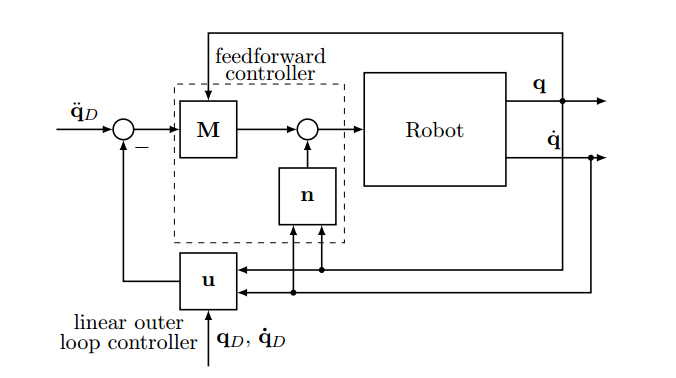
\includegraphics[width=0.65\textwidth]{pics/ct_controller.png}\\
	\caption{Controller overview of Computed Torque like controller with gravity compensation}
	\label{fig:ctLike_overview}
\end{figure}

The controller is designed similar to the Computed Torque PD-Controller, with a coefficient comparison of the characteristic polynomial. For the damping a critical damping is required and for the frequency of the system $\omega_n$ two different values are chosen, 100 ${rad \over s}$ and 10 ${rad \over s}$.\\
Figure \ref{fig:ctLike_pd1} shows the simulation with 100${rad \over s}$. The system reaches zero steady-state error within 0.2seconds. Therefore the initial torque has a peak of around 1kNm, which is in a range, where it is unreasonable to use motors, which are supporting this high torque. \\
In comparison the controller with $\omega_n = 10 {rad \over s} $ which is shown in figure \ref{fig:ctLike_pd2} does show reasonable values for the torque. The torques needed for this controller oscillate around 30Nm/10Nm with an amplitude of 20Nm/10Nm.\\
Although a lot of system components have not been used for the controller design, the controller show reasonable results, which are accurate enough for the most real world tasks.

\begin{figure}[]
	\centering
	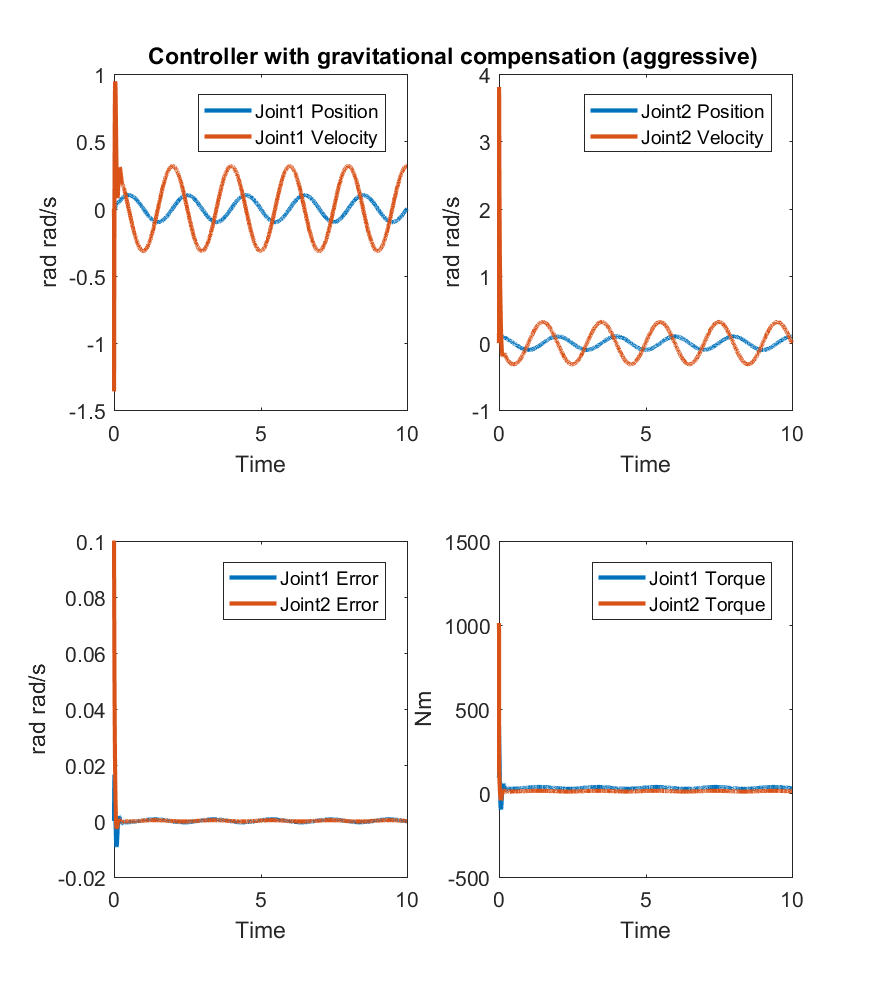
\includegraphics[width=0.85\textwidth]{pics/Controllerwithgravitationalcompensation(aggressive).png}\\
	\caption{Aggressive Computed Torque like controller with gravitational compensation}
	\label{fig:ctLike_pd1}
\end{figure}

\begin{figure}[]
	\centering
	\includegraphics[width=0.85\textwidth]{pics/Controllerwithgravitationalcompensation(moderate).png}\\
	\caption{Moderate Computed Torque like controller with gravitational compensation}
	\label{fig:ctLike_pd2}
\end{figure}

\section{Classical PD Joint Control}

The concept of classical joint controller further simplifies the model and even removes the gravitational model from the system. So the control law is given by:
\begin{equation*}
	\tau_c = -\mathbf{u}
\end{equation*}
The controller consists of two decoupled controller, one for each joint, they do not share any information or states, which might affect each offer. This approach is useful if the motor of robot arm uses a high gear ratio, since the gear reduces the influence of the non linear parts of the system. For motors with a high gear ration the problem from controlling a robot arm shifts to the controlling of the motor, which is easier to accomplish, since the motor itself is not changed, if the arm has some unknown disturbance.\\
For the controller design of the the PD-Controller a general second order polynomial is used. Again, critical damping is assumed during the controller design. The last free parameter $\omega_n$ is varied over different simulations. The used set of parameters is given in the following table:\\[1cm]

\begin{table*}[h]
	\begin{center}
		
		\label{tab:ch3_pd}
		\begin{tabular}{llll}
			& & & According \\
			& $k_{p,i}$ & $k_{d,i}$ & Figure \\
			\midrule
			$\omega_n = 10\,\mathrm{\frac{rad}{s}}$: & 100 & 20 & \ref{fig:ch3_sim21} \\
			$\omega_n = 25\,\mathrm{\frac{rad}{s}}$: & 625 & 50 & \ref{fig:ch3_sim22} \\
			$\omega_n = 50\,\mathrm{\frac{rad}{s}}$: & 2500 & 100 & \ref{fig:ch3_sim23} \\
			\bottomrule
		\end{tabular}
	\caption{Controller parameters for simulations witch classical PD controller}
	\end{center}
\end{table*}

The first simulation, figure \ref{fig:ch3_sim21}, show the results with $\omega_n$ = 10. Here the error of the joints is relatively large. This huge error is caused by absence of he gravity within the design process. Therefore the torques of the joints do not show any peak.\\

\begin{figure}[h]
	\centering
	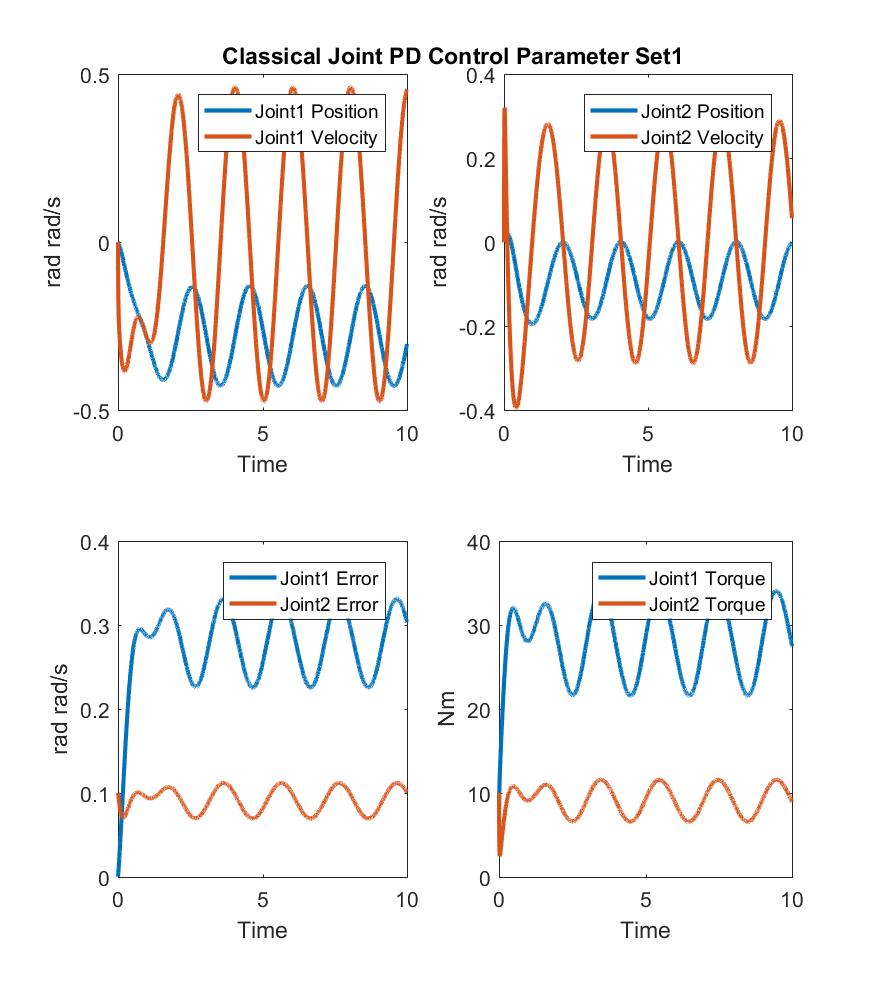
\includegraphics[width=0.85\textwidth]{pics/ClassicalJointPDControlParameterSet1.png}\\
	\caption{Classical PD Joint Control $\omega_n$ = 10}
	\label{fig:ch3_sim21}
\end{figure}

The next parameter set, figure \ref{fig:ch3_sim22}, does provide way less position error of the axes. Although the torques do have peaks at the beginning of around 60 Nm. After the initial peak the values of the torque decreases to same level as the previous simulation.

\begin{figure}[h]
	\centering
	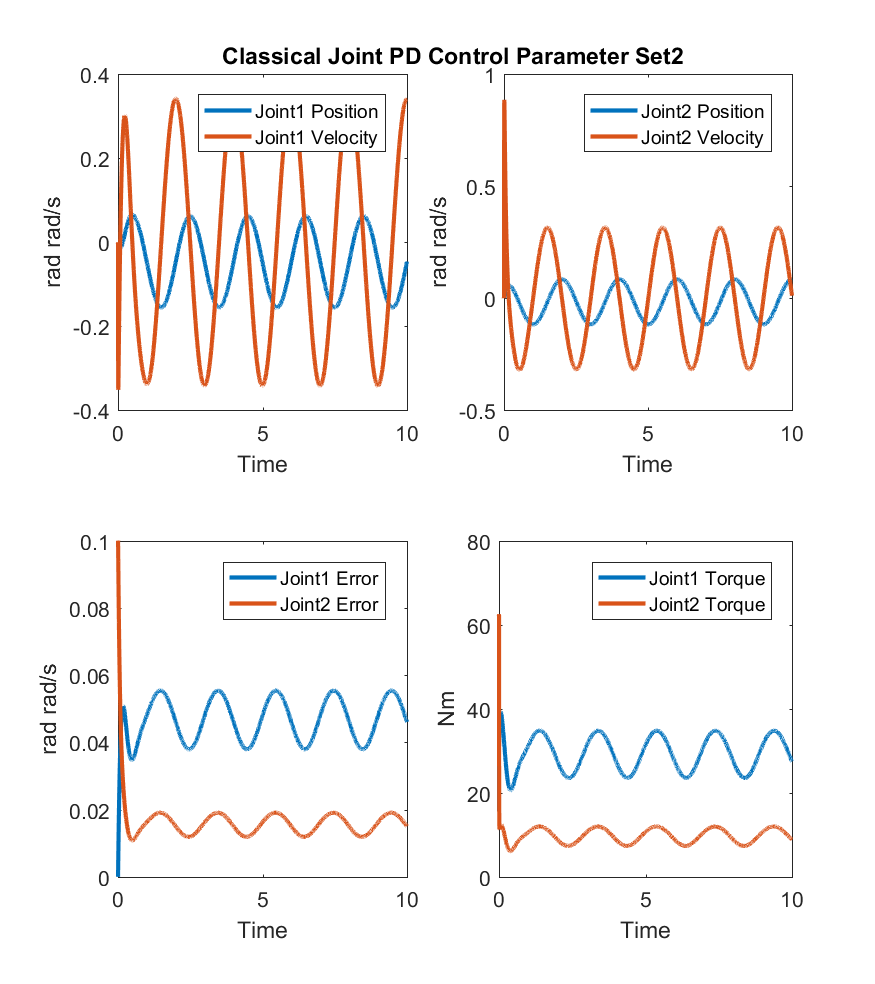
\includegraphics[width=0.85\textwidth]{pics/ClassicalJointPDControlParameterSet2.png}\\
	\caption{Classical PD Joint Control $\omega_n$ = 25}
	\label{fig:ch3_sim22}
\end{figure}

The last simulation uses the highest gains. Here an even higher peak torque is expected in comparison to the previous simulation. This expectation is valid, if the results from the last simulation is observed \ref{fig:ch3_sim23}. The initial peak of the torque is around 250Nm. But this controller provides with its more aggressive parameter set an even more accurate tracking of the reference and the position error is reduced to arounf 0.01rads.
\begin{figure}[h]
	\centering
	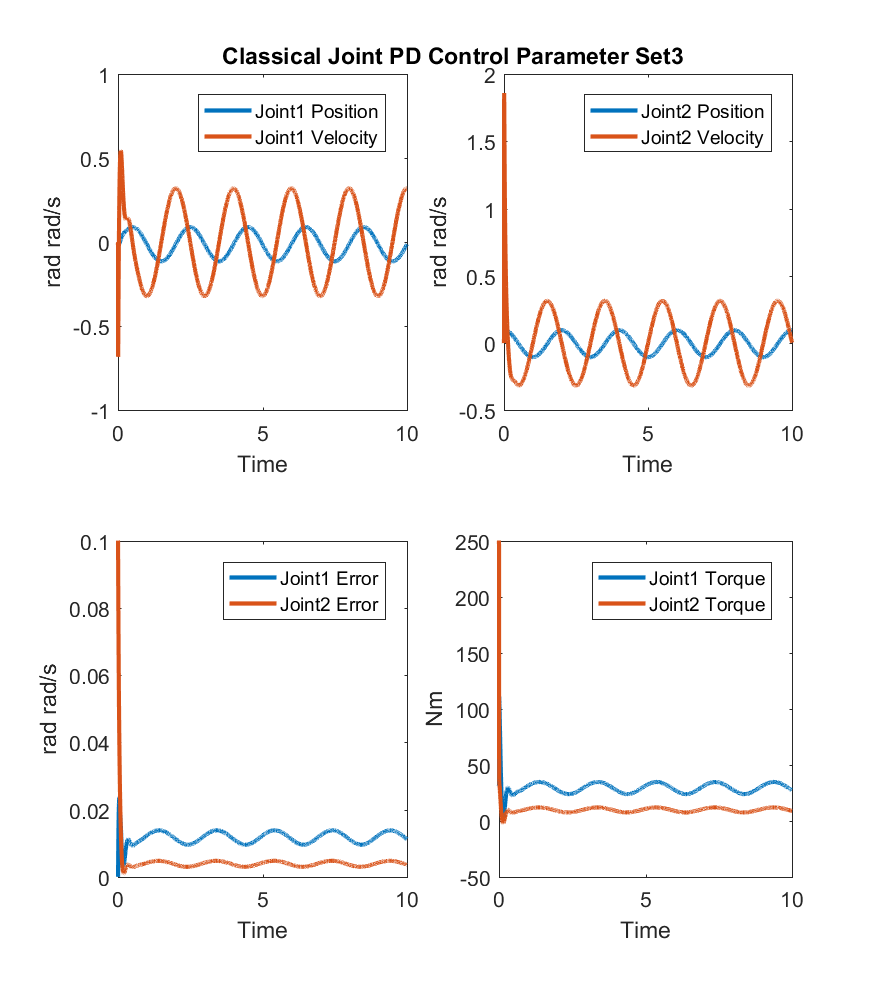
\includegraphics[width=0.85\textwidth]{pics/ClassicalJointPDControlParameterSet3.png}\\
\caption{Classical PD Joint Control $\omega_n$ = 50}
	\label{fig:ch3_sim23}
\end{figure}


\section{Classical PID Joint control}

All controllers from the previous section are not able to reach a steady-state error of zero. All controllers have an error unequal to zero even after longer time. This can be explained with the absence of the gravitational force within the design process. Anyway this errors, can be reduced taken into consideration and an integrator can be added to the controller. This integrator is able to take care of the gravitational term and compensate it.\\

By taking the characteristic polynomial of this controller:
\begin{equation*}
\Delta(s) = J_i s^3 + (B_i + k_{d,i}) s^2 +  k_{p,i} s + k_{i,i}
\end{equation*}

To find the stability region for the controller parameters, the Routh-Hurwitz stability criterion is applied.
\begin{gather*}
\begin{tabular}{>{$}c<{$}>{$}c<{$}>{$}c<{$}}
J & k_{p} & 0 \\
B + k_{d} & k_{i} & 0\\
\dfrac{(B + k_{d})k_{p}-J k_{i}}{B_i + k_{d}} & 0 & 0\\
k_{i} & 0 & 0
\end{tabular}
\end{gather*}

Since the inertia is always positive the following conditions have to be fulfilled so that the closed loop controller is stable.
\begin{align*}
B + k_{d} &> 0\\
k_{i} &> 0\\
(B + k_{d})\frac{k_{p}}{J} &> k_{i}
\end{align*}

This controller is used with 3 different set of gains. First with some moderate controller gains, second some aggressive controller gains and last the aggressive controller with some saturation within the torque. The saturation is simulated to match a real world hardware better, which is not able to supply infinite values of torque. The overview over the parameters is given within the next table:
\begin{table}[h]
	\begin{center}
		
		\begin{tabular}{lllll}
			& & & & According \\
			& $k_{p}$ & $k_{d}$ & saturation & Figure \\
			\midrule
			$\omega_n = 10\,\mathrm{\frac{rad}{s}}$: & 300 & 30 & $\pm\infty\,\mathrm{N\,m}$ & \ref{fig:ch3_sim31} \\
			$\omega_n = 50\,\mathrm{\frac{rad}{s}}$: & 2540 & 100.4 & $\pm\infty\,\mathrm{N\,m}$ & \ref{fig:ch3_sim32} \\
			$\omega_n = 50\,\mathrm{\frac{rad}{s}}$: & 2540 & 100.4 & $\pm 35\,\mathrm{N\,m}$ &  \ref{fig:ch3_sim33}\\
			\bottomrule
		\end{tabular}
	\caption{Controller parameters for simulations witch classical PID controller}
	\end{center}
\end{table}

\begin{figure}[h]
	\centering
	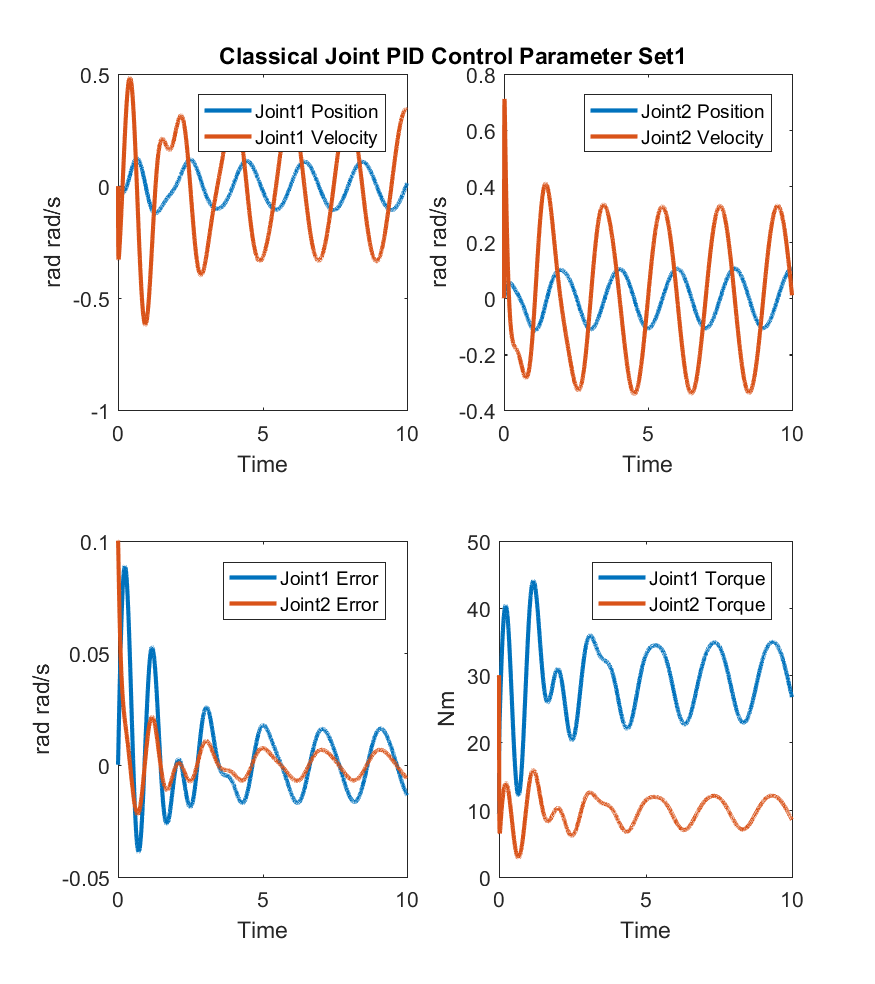
\includegraphics[width=0.85\textwidth]{pics/ClassicalJointPIDControlParameterSet1.png}\\
	\caption{Classical PD Joint Control $\omega_n$ = 10}
	\label{fig:ch3_sim31}
\end{figure}

In figure \ref{fig:ch3_sim31} the simulation with the moderate parameter set can be seen. Here the constant offset of the error has been removed and the error oscillates around zero. Although the amplitude of the error is rather high with 0.1rads.
\begin{figure}[h]
	\centering
	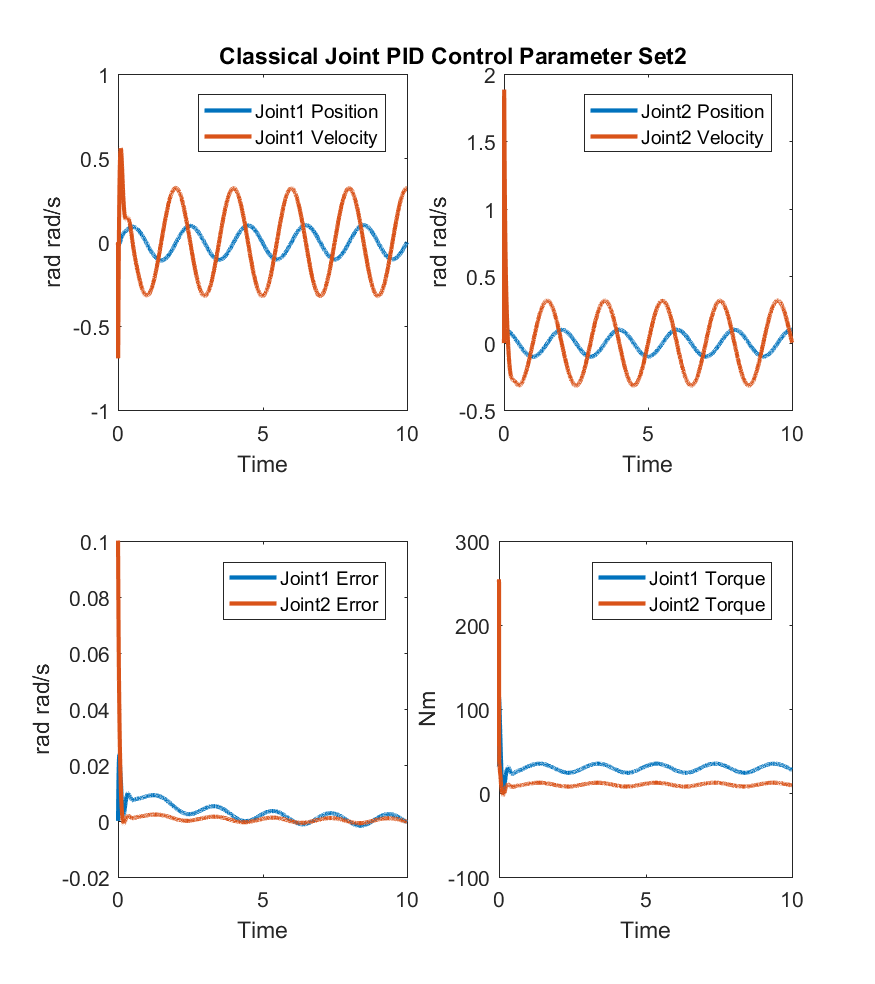
\includegraphics[width=0.85\textwidth]{pics/ClassicalJointPIDControlParameterSet2.png}\\
	\caption{Classical PID Joint Control $\omega_n$ = 50}
	\label{fig:ch3_sim32}
\end{figure}

In the next simulation which can be seen within figure \ref{fig:ch3_sim32} the dynamics of the error are greatly improved in comparison to the previous simulation. This can be explained by the way more aggressive parameter set. The drawback of this parameter set is the high initial peak within the torque. The max value of the torque is around 250Nm. Which makes this controller not really suitable for a real world implementation.
\begin{figure}[h]
	\centering
	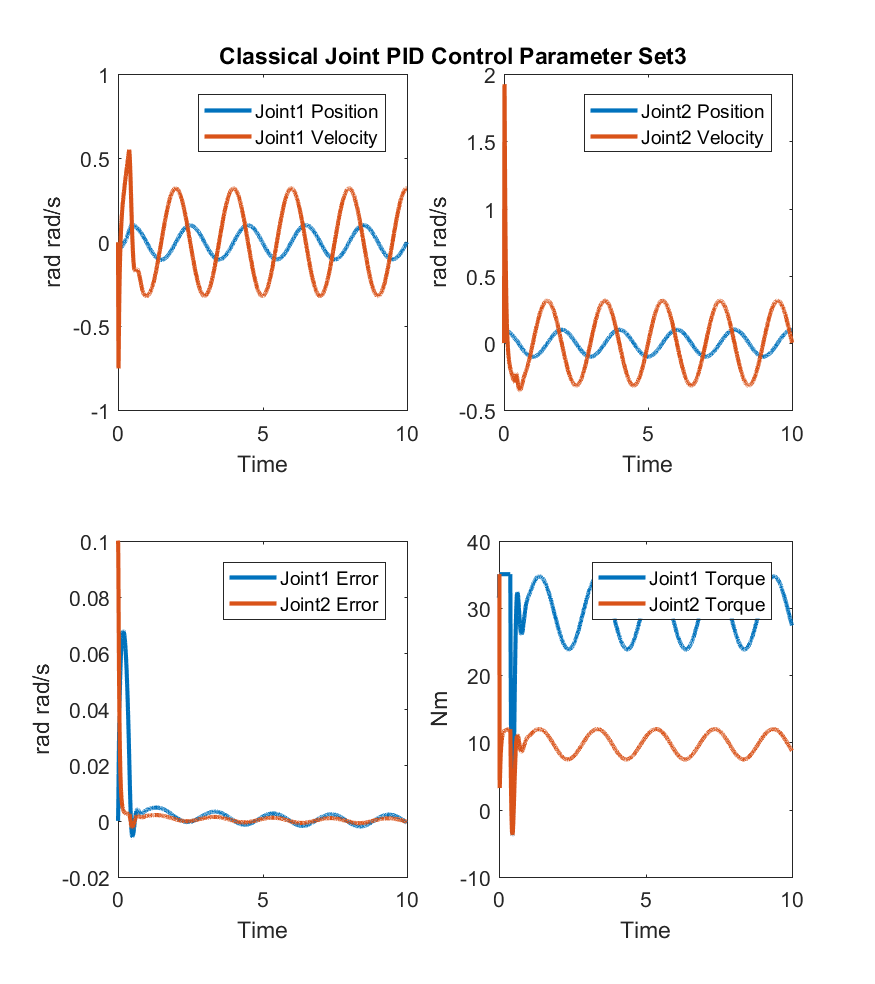
\includegraphics[width=0.85\textwidth]{pics/ClassicalJointPIDControlParameterSet3.png}\\
	\caption{Classical PID Joint Control $\omega_n$ = 50 with saturation}
	\label{fig:ch3_sim33}
\end{figure}
The last simulation of the PID joint controllers, will utilize the previous parameter set, which has shown suitable system dynamics, although it has high torque peaks. This simulation will saturate the torque signal at $\pm$35Nm. The saturation is clearly visible within the simulation results. Comparing the error dynamics of the last simulation with the error from the previous one, there is almost no difference visible. So it can be said that the PID joint control is a suitable method for the control of a robot arm. The saturation itself does not provide any drawback and is usually automatically implemented within the motor driver.

\chapter{ Practical issues at the realisation of robot control}

 When a controller for a robot needs to be implemented often a digital controller is needed. For the design of a discrete CT Controller the dynamics of the robot needs to be discretized, which leads to a very complicated system description and a even more complicated controller design. Since the CT Controller is a non-linear one, you cannot just discretize the controller and expect the same result. The only reasonable method is to use the discretized version of the CT controller as an approximation. For the following simulation and discretized version of a computed torque PD-controller will be used in a digital implementation. The robot arm itself will be still simulated with a variable step solver to contain the continuous behavior of the robot. The real world robot model is also a continuous one, so the behavior of the controller can be simulated within a good framework.\\
 The parameter of the controller will be the same as the computed torque PD-Controller with critical damping \ref{fig:ct_pd1}. For this simulation the sampling time of the controller will be changed from  1ms, 50ms and 100ms. The rest of the simulation model will run with a variable step solver.
 
 \begin{figure}[h]
 	\centering
 	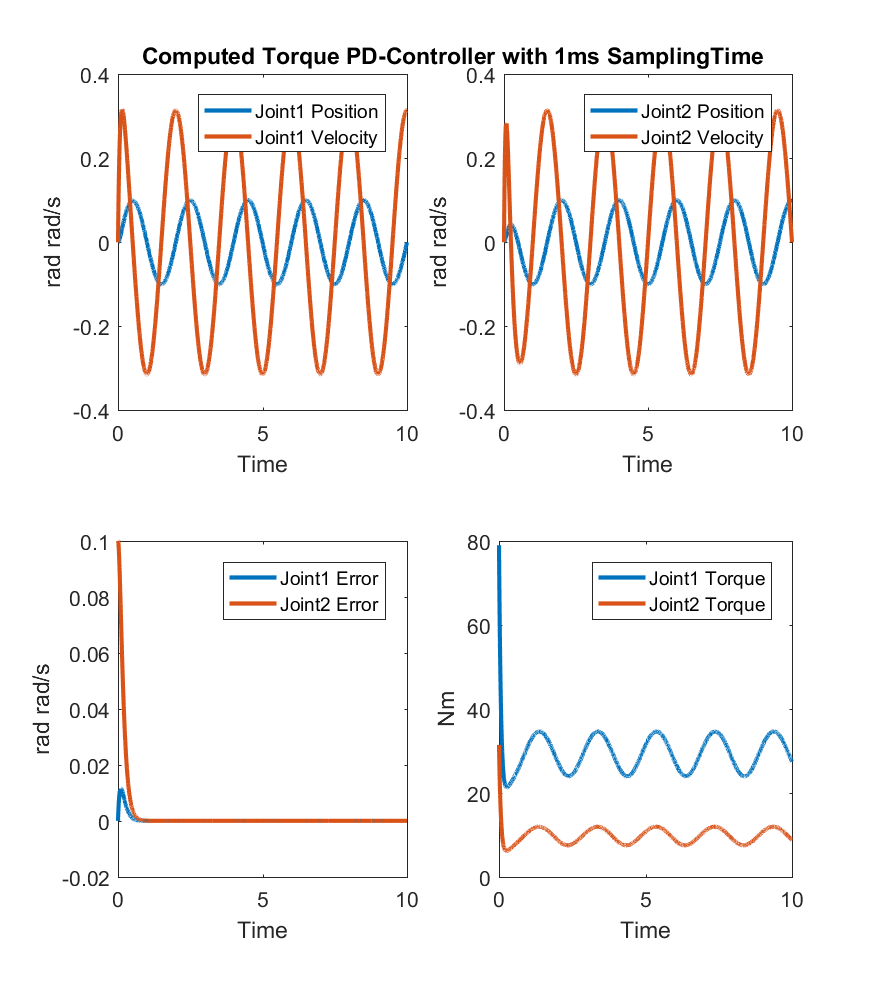
\includegraphics[width=0.85\textwidth]{pics/ComputedTorquePD-Controllerwith1msSamplingTime.png}\\
 	\caption{Discrete CT-PD Controller with $T_s$ = 1ms}
 	\label{fig:ch3_digi1}
 \end{figure}

The first simulation, which can be seen in figure \ref{fig:ch3_digi1}, show about the same behavior as the continuous implementation. 
\begin{figure}[h]
	\centering
	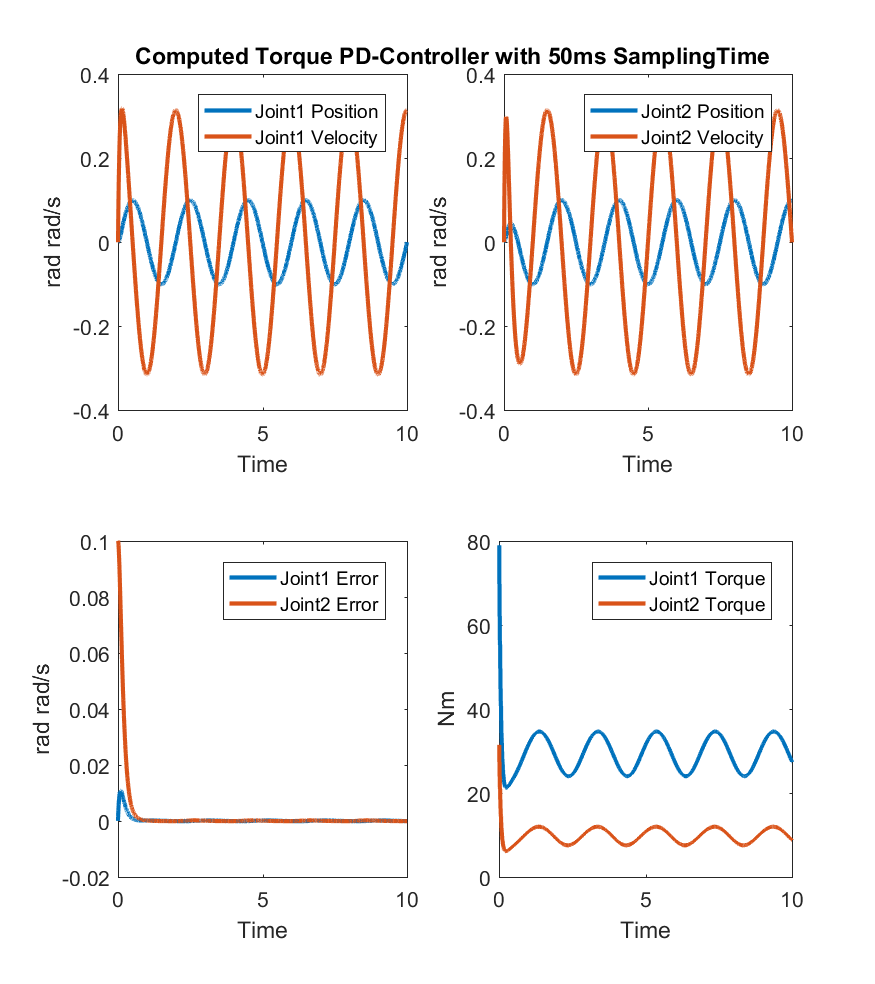
\includegraphics[width=0.85\textwidth]{pics/ComputedTorquePD-Controllerwith50msSamplingTime.png}\\
	\caption{Discrete CT-PD Controller with $T_s$ = 50ms}
	\label{fig:ch3_digi2}
\end{figure}
 The next simulation with a sampling time of 50ms, figure \ref{fig:ch3_digi2}, starts to show some differences to the continuous implementation. The error signal has some minor oscillations. All of the are still pretty small and neglect-able for the most application. 
\begin{figure}[h]
	\centering
	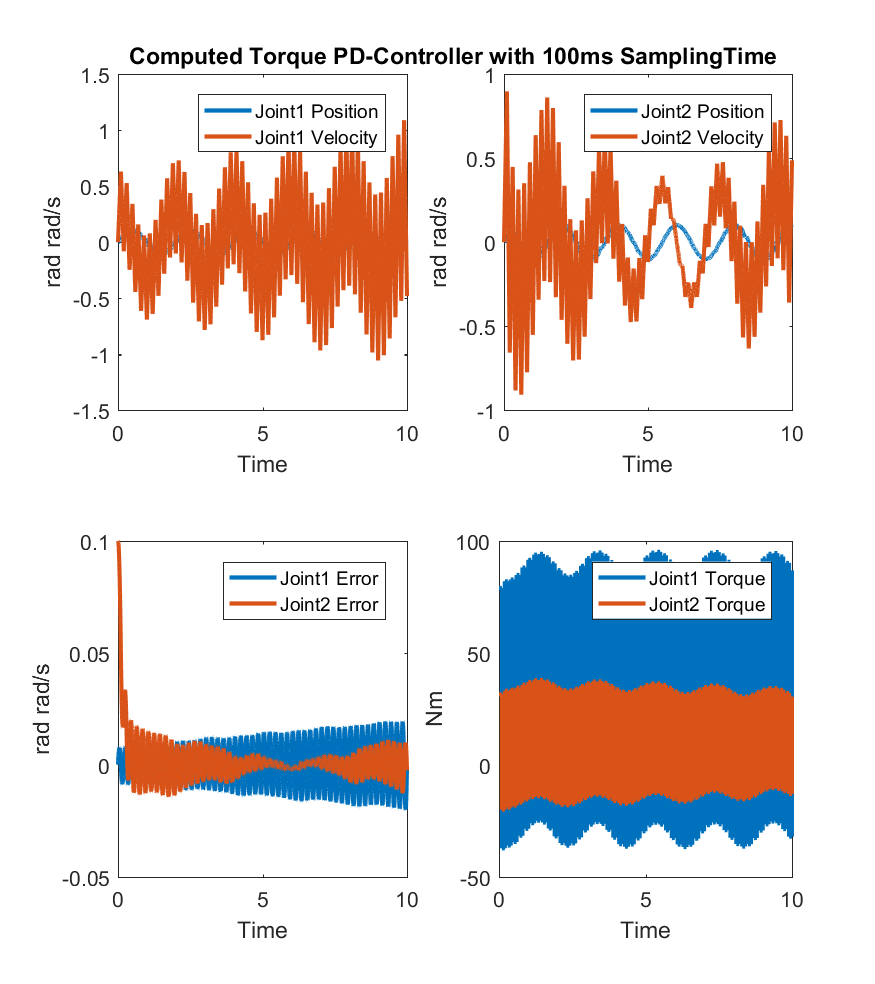
\includegraphics[width=0.85\textwidth]{pics/ComputedTorquePD-Controllerwith100msSamplingTime.png}\\
	\caption{Discrete CT-PD Controller with $T_s$ = 100ms}
	\label{fig:ch3_digi3}
\end{figure}
 
 If the sample time of the controller is further increased the controller starts to be unstable. This can be seen in figure \ref{fig:ch3_digi3}. Here the controller itself is too slow to react on any changes of the model. Until the controller is calculated again the model has already moved so far, that the control action needs to be inverted. This leads to an oscillation with increasing amplitude.
\chapter{ Computed Torque like Controller with disturbance estimator}

Similar to the classical joint control, this controller is a completely decoupled controller, which control each joint independent and separately. In comparison to the classical joint control, which neglected all nonlinearities, this controller estimates the non linearities within the system for each joint. The controller consists of the average moment of inertia of the corresponding joint, a PD controller for the stabilization and the disturbance estimator to compensate for unknown or unmodelled system dynamics.

\begin{gather*}
\tau_{c,i} = \bar{M}_{i}\ddot{q}_{calc}+ \hat{w}(q,\dot{q})
\intertext{where:}
\begin{tabular}{>{$}l<{$} @{${}:{}$} l}
\bar{M}_{i}             & average moment of inertia of the joint         \\
\ddot{q}_{calc}        & $\ddot{q}_{D} + k_{d}\dot{e}+k_{p}e$ \\
\hat{w}(q,\dot{q}) & estimated disturbances
\end{tabular}\nonumber
\end{gather*}

For the estimation of the disturbances, a PI estimator of the following form is used:

\begin{gather*}
\hat{w}(q,\dot{q}) = l(\dot{q}_{calc} - \dot{q})
\label{eq:eq1}
\intertext{where:}
\begin{tabular}{>{$}l<{$} @{${}:{}$} l}
l & estimator parameter
\end{tabular}\nonumber
\end{gather*}

The controller structure can be seen in figure \ref{fig:ctEstimator}.
\begin{figure}[]
	\centering
	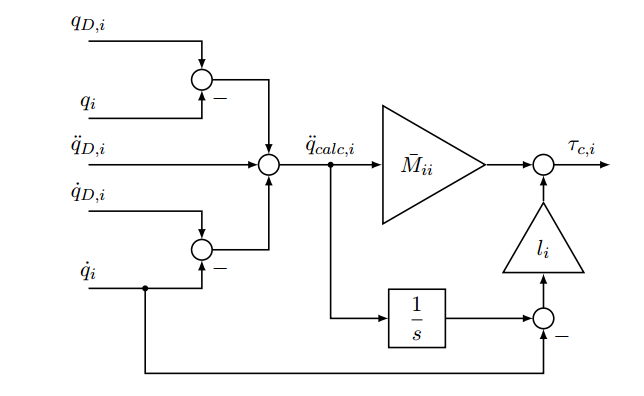
\includegraphics[width=0.55\textwidth]{pics/ctestimator.png}\\
	\caption{Controller overview of Computed Torque like controller with distortion estimator}
	\label{fig:ctEstimator}
\end{figure}

For the simulation of this controller several different parameter sets are used, which can be seen within table \ref{tab:ch5_distesti}.

\begin{table}[h]
	\begin{center}
		
		\label{tab:ch5_distesti}
		\begin{tabular}{lll}
			&                                   & According          \\
			$l_i$ & $\frac{\omega_{estim}}{\omega_n}$ & Figure             \\
			\midrule
			20    & 2                                 & \ref{fig:ch4_esti1} \\
			100   & 2                                 & \ref{fig:ch4_esti2} \\
			100   & 10                                & \ref{fig:ch4_esti3} \\
			\bottomrule
		\end{tabular}
	\caption{Controller parameters for simulations witch CT like controller with disturbance estimator}
	\end{center}
\end{table}

Figure \ref{fig:ch4_esti1} show the first simulation result. Here the controller needs around 20 seconds to settle and the initial peak of the torque is around 100Nm.\\
\begin{figure}[]
	\centering
	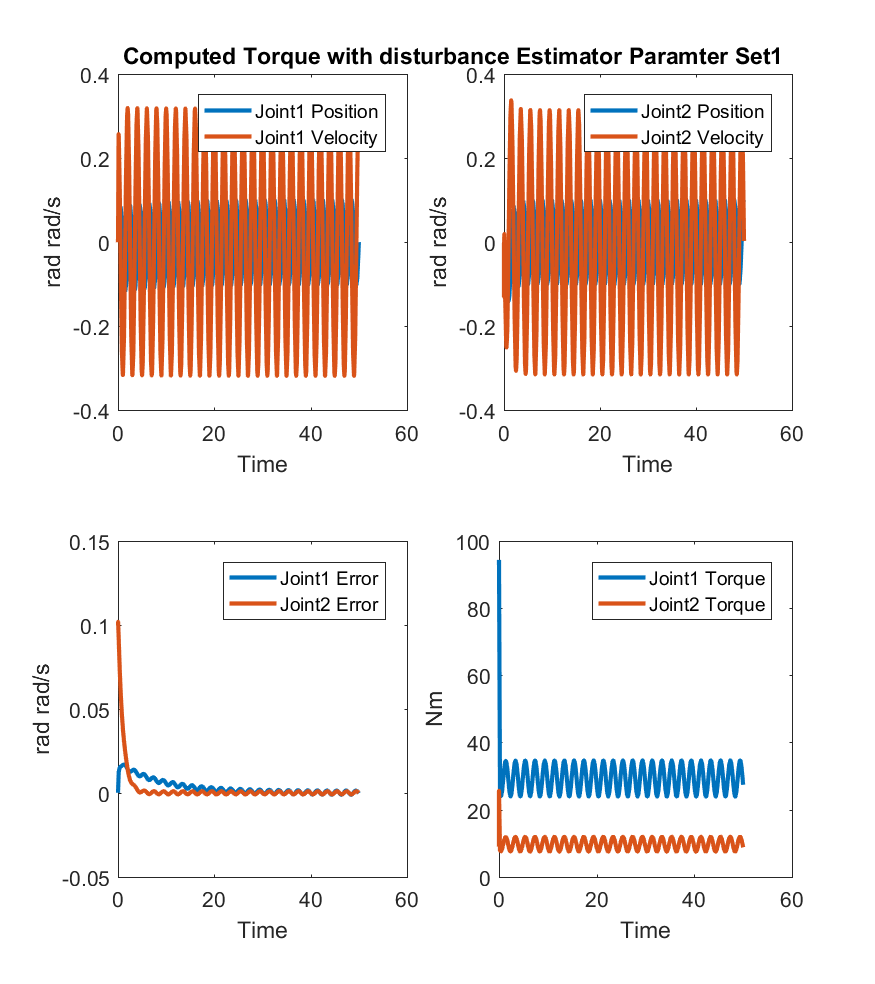
\includegraphics[width=0.85\textwidth]{pics/ComputedTorquewithdisturbanceEstimatorParamterSet1.png}\\
	\caption{CT like Controller with disturbance estimator}
	\label{fig:ch4_esti1}
\end{figure}
The next simulation uses parameters with higher gains, which lead to a settling time of around 2seconds; figure \ref{fig:ch4_esti2}. To reach the faster result a higher peak of the torque is needed.
\begin{figure}[]
	\centering
	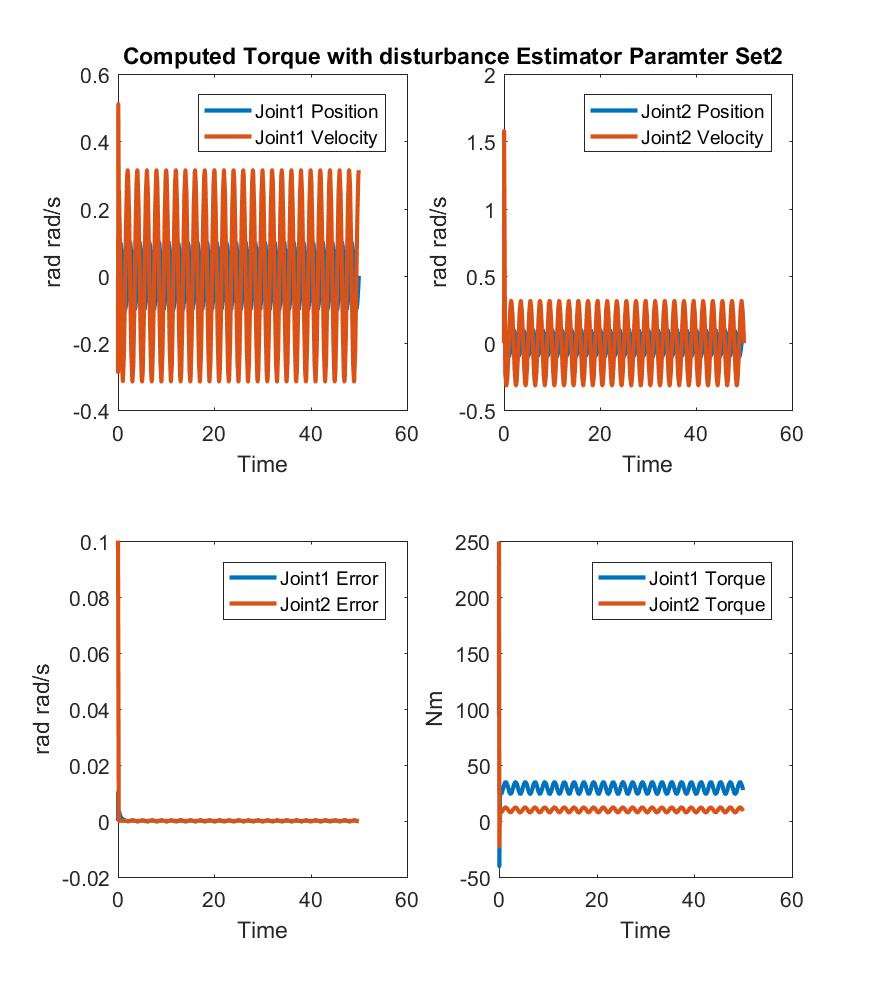
\includegraphics[width=0.85\textwidth]{pics/ComputedTorquewithdisturbanceEstimatorParamterSet2.png}\\
	\caption{CT like Controller with disturbance estimator}
	\label{fig:ch4_esti2}
\end{figure}

The last parameter set combines the advantages from the previous simulations. It has a fast settling at around 5seconds, which is short compared to the first simulation. And the torque of the system does not show similar peaks as the previous simulation with a maximum of around 100Nm.
\begin{figure}[]
	\centering
	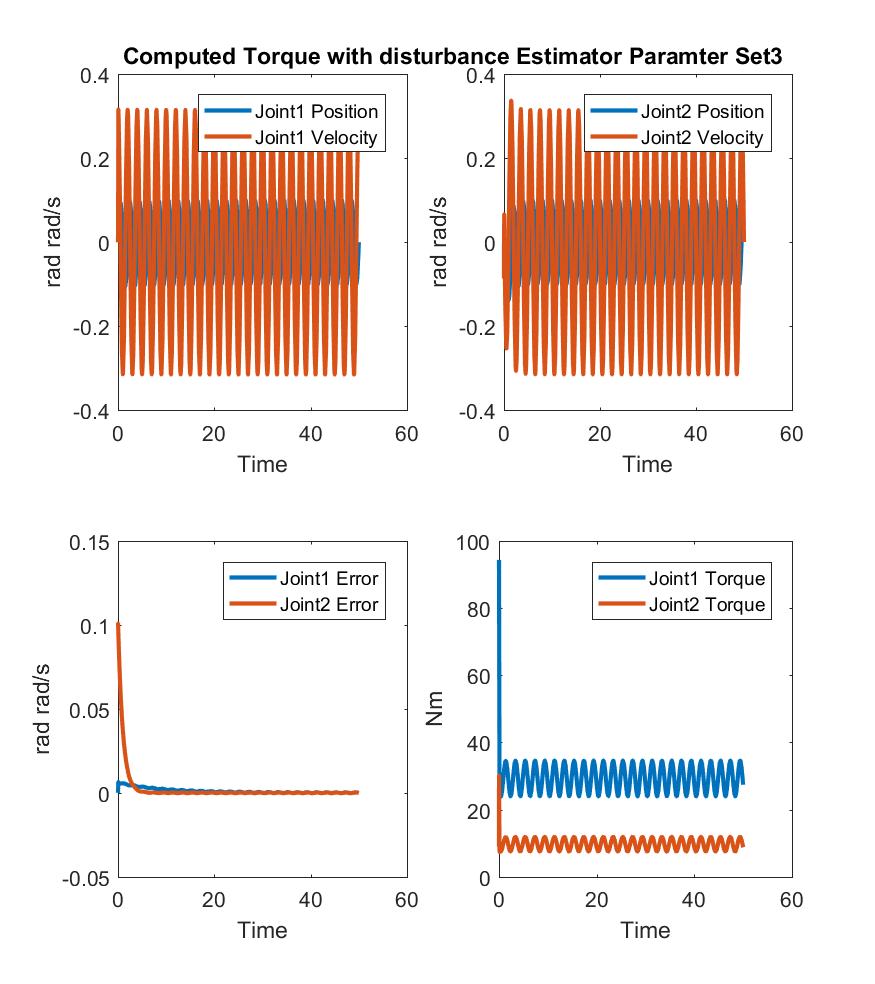
\includegraphics[width=0.85\textwidth]{pics/ComputedTorquewithdisturbanceEstimatorParamterSet3.png}\\
	\caption{CT like Controller with disturbance estimator}
	\label{fig:ch4_esti3}
\end{figure}


\chapter{ Sliding Mode controller}

The idea behind sliding mode is to force the states of a system to a so called sliding manifold and let it slide along this surface to the origin. When the states are on the surface the system show reduced order dynamics. To keep the system on the manifold a high frequency switching signal is needed. This can be obtained easily with a sign. As this would need to infinite fast switching , which cannot be realized, a boundary layer is introduced. This layer is achieved by using, instead of sign-function, another function like tanh.\\
To stabilize the error system of the robot arm the following sliding manifold is used:
\begin{gather*}
\mathbf{s} = \dot{\mathbf{e}} + \Lambda \mathbf{e}
\intertext{where:}
\begin{tabular}{>{$}l<{$} @{${}:{}$} l}
	\Lambda & diagonal matrix with time constants of the systems, when in sliding mode
\end{tabular}\nonumber
\end{gather*}

This system corresponds to a first order differential equation. To be stable the eigenvalues of this system needs to be negative. To control the robot the following control law is used:
\begin{gather*}
\tau_c = \hat{\mathbf{M}}\ddot{\mathbf{q}}_s + \hat{\mathbf{V}}_m \dot{\mathbf{q}}_s + \hat{\mathbf{g}} + \mathbf{K} sign(\mathbf{s})
\intertext{where:}
\begin{tabular}{>{$}l<{$} @{${}:{}$} l}
\hat{\mathbf{M}} & estimated inertia matrix\\
\hat{\mathbf{V}}_m & estimated centrifugal/coriolis matrix\\
\dot{\mathbf{q}}_s & $\Lambda \mathbf{e} + \mathbf{\dot{q}}_D$\\
\hat{\mathbf{g}} & estimated gravitation vector\\
\mathbf{K} & diagonal matrix with gains
\end{tabular}\nonumber
\end{gather*}

The parameter $\mathbf{K}$ is used to compensate for the unknown or unmodelled dynamics. The better the model is the smaller this parameter can be chosen.
For the simulation following parameter sets have been chosen: 
\begin{table}[h]
	\begin{center}
		\label{tab:smo}
		\begin{tabular}{lllll}
			&     &							 &Switching& According          \\
			$\lambda$ & $k$ &$\hat{\mathbf{g}}$&Function& Figure             \\
			\midrule
			10    & 20 &$0.75\mathbf{g}  $& sign(s)& \ref{fig:ch5_smo1} \\
			10    & 10 &$0.75\mathbf{g}  $& sign(s)& \ref{fig:ch5_smo2} \\
			25    & 20 &$0.75\mathbf{g}  $& sign(s)& \ref{fig:ch5_smo3} \\
			10    & 20 &$0\mathbf{g}  $& sign(s)& \ref{fig:ch5_smo4} \\
			10    & 30 &$0\mathbf{g}  $& sign(s)& \ref{fig:ch5_smo5} \\
			10    & 20 &$0\mathbf{g}  $& tanh(s)& \ref{fig:ch5_smo6} \\
			10    & 40 &$0\mathbf{g}  $& tanh(5s)& \ref{fig:ch5_smo7} \\
			\bottomrule
		\end{tabular}
		\caption{Controller parameters for simulations with sliding mode controller}
	\end{center}
\end{table}
\chapter{ Computed Torque like Controller with disturbance estimator}

%\include{Theory}
%\include{Identification}
%\include{Analysis}
%\include{Conclusion}
%\bibliography{bibliography}
%\include{Statement}

%%% Neues Kapitel %%%
%\chapter{Kapitel}
%\label{sec:Kapitel}
%
%\section{Unterpunkt}

%%% Bild einfügen (nur .eps) %%%
%\begin{figure}[h]
%	\centering
%	\includegraphics[width=0.85\textwidth]{pics/xyz}\\
%	\caption{Parameter Sweep für die Weite des NMOS4}
%	\label{fig:xyz}
%\end{figure}
% Simulink_Modell_Prints('name_simulink_datei','p')

%%% Tabelle einfügen
%\begin{table}[h]
%	\begin{center}
%		\caption{SPICE Parameter für NMOS und PMOS} 
%		\begin{tabular}{|l|l|l|}
%			\hline
%			x & y & z\\
%			\hline
%		\end{tabular}
%		\label{tab:}
%	\end{center}
%\end{table}

%%% Formel einfügen
%\begin{equation}
%	\centering
%	Formel
%	\label{eq:}
%\end{equation}

\end{document}
